\section{Introducción}\label{sec:introduccion}

% Reinforcement Learning
\subsection{Aprendizaje por Refuerzo}\label{subsec:aprendizaje-por-refuerzo}

El aprendizaje por refuerzo, \textit{RL} por sus siglas en inglés, es un área del \textit{aprendizaje automático} que estudia cómo un agente aprende a tomar decisiones óptimas interaccionando con un entorno para alcanzar un objetivo a largo plazo.
A diferencia de otros enfoques de aprendizaje automático, el paradigma en cuestión no requiere de un conjunto de datos o modelos del entorno.
En cambio, el agente aprende a través de la experiencia, recibiendo penalizaciones o recompensas por la acción tomada.

Entre los subelementos de un sistema de aprendizaje por refuerzo se encuentran: \textit{política}, \textit{recompensa}, \textit{función de valor} y (opcionalmente) un \textit{modelo del entorno}.
La \textit{política} es una función que mapea un estado a una acción, es decir, determina la acción a tomar en un estado dado.
La \textit{recompensa} es una señal que indica al agente si la acción tomada fue correcta o no.
La \textit{función de valor} es una función que estima la recompensa esperada de un estado o acción, es decir, determina la recompensa que el agente puede acumular en el futuro, dado un estado.
Por último, el \textit{modelo} es una representación del entorno que el agente puede usar para simular el comportamiento del entorno dado un estado y acción~\cite{Sutton2018}.
Los modelos de aprendizaje reforzado pueden clasificarse en dos categorías principales:

\textbf{Aprendizaje por Refuerzo Basado en Modelo}
\textit{MBRL} por sus siglas en inglés, los cuales usan las interacciones con el entorno para aprender un modelo del entorno y, posteriormente, lo usa para planificar una política.
La representación interna del entorno le permite predecir el comportamiento del mismo y tomar decisiones óptimas.
En general, este enfoque es más eficiente, ya que aprender una política directamente no es necesariamente más eficiente que aprender un modelo y planificar una política~\cite{Sutton2018, benchmarking_2019, YiWan_2022, MuZero_2020}.
Por otro lado, el aprendizaje basado en modelos se ha popularizado por su menor complejidad de muestreo.
Además, han incorporado técnicas de ensambles y modelos probabilísticos para aliviar el problema de \textit{sesgo-varianza} y alcanzar el rendimiento del aprendizaje por refuerzo sin modelo~\cite{benchmarking_2019}.

\paragraph{Aprendizaje por Refuerzo sin Modelo}
\textit{MFRL} por sus siglas en inglés, aprenden una función de valor o política directamente de la interacción con el entorno.
La función asigna un valor para cada par \textit{estado-acción}, sin necesidad de modelar el entorno en sí mismo, la función en cuestión se utiliza para seleccionar la acción que maximice la recompensa en el largo plazo~\cite{benchmarking_2019, Sutton2018}.
Por otro lado, el método en cuestión es el enfoque más popular en la actualidad, incluso se usa como bloque de construcción en aprendizaje por refuerzo basado en modelos~\cite{Sutton2018}.
No obstante, su aplicación se encuentra reducida a entornos simulados, dada su alta complejidad de muestreo.

La figura~\ref{fig:MFRL_MBRL_diagram} ilustra las relaciones entre la experiencia, el modelo, la función de valor y la política en un contexto de aprendizaje por refuerzo con y sin modelo.

\begin{figure}[H]
    \centering
    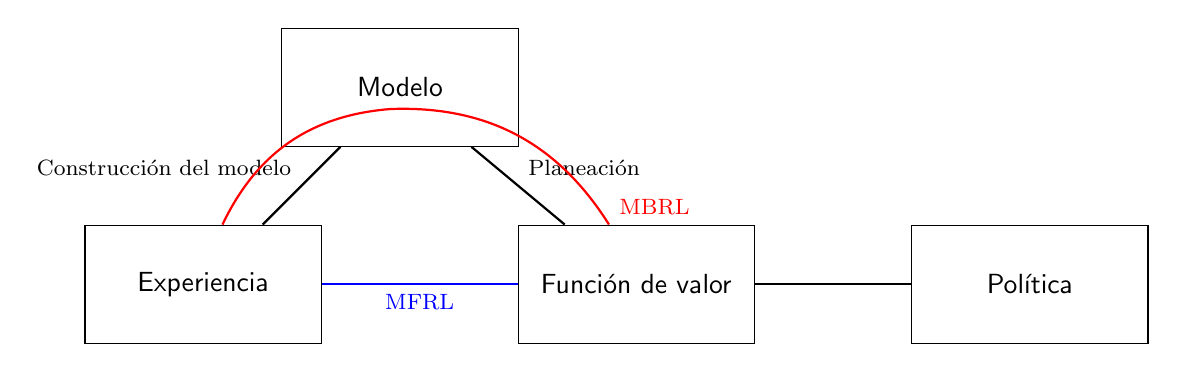
\begin{tikzpicture}[
        box/.style={rectangle, draw, minimum width=3cm, minimum height=1.5cm, align=center},
        arrow/.style={thick},
        every node/.style={font=\sffamily}
    ]

        % Nodes
        \node (model_1) at (2.5,-0.25) {};
        \node[box] (model) at (2.5,0) {Modelo};
        \node[box] (experience) at (0,-2.5) {Experiencia};
        \node[box] (value) at (5.5,-2.5) {Función de valor};
        \node[box] (policy) at (10.5,-2.5) {Política};

        % Arrows
        \draw[arrow] (experience) -- (model) node[midway, above left, font=\footnotesize] {Construcción del modelo};
        \draw[arrow] (model) -- (value) node[midway, above right, font=\footnotesize] {Planeación};
        \draw[arrow, blue, thick] (experience) -- (value) node[midway, below, font=\footnotesize] {MFRL};
        \draw[arrow, red, thick, bend left=30] (experience) to (model_1) to (value) node[above right, font=\footnotesize] {MBRL};
        \draw[arrow] (value) -- (policy);

    \end{tikzpicture}
    \caption{Relaciones entre {experiencia}, {modelo}, {función de valor} y {política} en un contexto de aprendizaje por refuerzo con modelo (MBRL) y sin modelo (MFRL).}
    \label{fig:MFRL_MBRL_diagram}
\end{figure}

\subsection{El problema de la adaptabilidad}\label{subsec:el-problema-de-la-adaptabilidad}
A pesar de los avances en el aprendizaje por refuerzo y las expectativas generadas en la comunidad, aún no se cuenta con métodos estandarizados para comparar un modelo de aprendizaje por refuerzo con otro, tampoco se encuentran lineamientos que fijen una ruta para la evaluación de nuevos modelos con respecto a los ya existentes.
Contar con una técnica de evaluación y comparación sistemática de modelos de aprendizaje por refuerzo, facilitaría el reconocimiento de ventajas y desventajas de un modelo y la elección de un modelo en función de las necesidades del problema a resolver y guiar a investigadores en la dirección de futuras investigaciones.
Además, se busca evaluar la adaptabilidad de los modelos para resolver tareas nuevas, que compartan características con las tareas para las que fueron entrenados inicialmente y, en consecuencia, evaluar la capacidad de generalización de los modelos~\cite{YiWan_2022, benchmarking_2019}.

En contraste, áreas como la visión por computadora cuentan con conjuntos de datos de código abierto y métricas estándar para evaluar el rendimiento de los modelos.
Por ejemplo, el conjunto de datos \textit{ImageNet} y la métrica \textit{Top-1 Accuracy}~\cite{imagenet}.
Ahora bien, el aprendizaje por refuerzo sin modelo cuenta con librerías como \textit{rllab}~\cite{rllab}, \textit{OpenAI Gym}~\cite{openai-gym} y \textit{Deepmind Control Suite}~\cite{deepmind-control-suite}, que permiten acceder a entornos y métodos de evaluación de modelos.
No obstante, no se encuentran soluciones similares para el caso de los modelos de aprendizaje por refuerzo basados en modelos~\cite{benchmarking_2019} dada la falta de librerías de código abierto que se asemejen al entorno de evaluación de modelos de aprendizaje por refuerzo sin modelo.

Actualmente, la comparación de modelos recae principalmente en la eficiencia de muestreo \textit{(sample-efficiency)} en una tarea específica, la cual se refiere a la capacidad de aprendizaje de un algoritmo en función de la cantidad de datos, o en el caso del aprendizaje por refuerzo, la cantidad de interacciones con el entorno~\cite{benchmarking_2019}.
La eficiencia de muestreo de única tarea es la métrica de facto para evaluar el aprendizaje reforzado basado en modelos.
No obstante, no es lo suficientemente robusta para evaluar el progreso en la investigación de aprendizaje por refuerzo basado en modelos.
Primero, no distingue las mejoras que la exploración y generalización aportan por separado.
Segundo, no proporciona una comparación clara con el caso ideal de un método basado en modelo.
Finalmente, el hecho de evaluarse en una sola tarea no mide la relevancia que el modelo puede tener al desempeñar tareas nuevas y/o en más de una tarea~\cite{LOCA_2020}.

\subsection{LoCA: Adaptación de Cambio Local}\label{subsec:loca-adaptacion-de-cambio-local}
En la búsqueda de una solución a los problemas planteados, se desarrolló LoCA \textit{(Local Change Adaptation regret)}, el cual provee una solución para medir qué tan rápido el modelo adapta su política ante cambios en el entorno, como lo es un cambio en la tarea a resolver.
El algoritmo en cuestión permite exponer modelos de aprendizaje reforzado, independiente de su funcionamiento interno, a cambios en la tarea a resolver y, en el caso de los métodos basados en modelos, estimar cuantitativamente cuán cerca se encuentra el modelo de un modelo ideal~\cite{LOCA_2020}.
El algoritmo consta de tres fases:

\paragraph{Fase 1: Pre-entrenamiento en la tarea \textit{A}}
\begin{itemize}
    \item \textbf{Objetivo}: Aprendizaje de una política estable, una función de valor y/o un modelo del entorno de acuerdo con la estructura de las recompensas.
    \item \textbf{Distribución de estados iniciales}: El agente se inicializa con estados iniciales aleatorios en el dominio del espacio de estados, lo que garantiza que el agente explora y aprende las dinámicas propias de la tarea \textit{A}.
    \item \textbf{Recompensas}: Se usa la función de recompensas $r_A$, diseñada para que la política óptima transicione al estado terminal $T_1$. Cuenta con un factor de descuento $0 < \gamma < 1$.
\end{itemize}

\paragraph{Fase 2: Pre-entrenamiento local en la tarea \textit{B}}
\begin{itemize}
    \item \textbf{Objetivo}: adaptar el agente y su conocimiento a una estructura de recompensas diferente, únicamente bajo experiencias locales. Al restringir la experiencia del agente a la zona $T_1$ el agente adapta su política teniendo en cuenta las experiencias locales.
    \item \textbf{Distribución de estados iniciales}: El entrenamiento comienza con la asignación de un estado inicial aleatorio en la zona $T_1$, se forza el agente a que no pueda escapar de la zona hasta terminar el episodio.
    \item \textbf{Recompensas}: Se usa la función de recompensas $r_B$ cuya recompensa por transicionar al estado $T_1$ se encuentra reducida, se busca que el agente encuentre el estado terminal $T_2$. Cuenta con un factor de descuento $0 < \gamma < 1$.
\end{itemize}

\paragraph{Fase 3: Entrenamiento y evaluación en la tarea \textit{B}}
\begin{itemize}
    \item \textbf{Objetivo}: Evaluar qué tan bien el agente adaptó su política a la nueva tarea \textit{B} después del pre-entrenamiento local en la \textit{Fase 2}, que a diferencia de dicha fase, se le permite explorar todo el espacio de estados mientras se entrena.
    \item \textbf{Distribución de estados iniciales}: Se permite al agente explorar todo el espacio de estados.
    \item \textbf{Recompensas}: Se mide la habilidad del agente para encontrar el estado terminal $T_2$ con un número finito de pasos desde un estado inicial definido.
\end{itemize}

En resumen, el arreglo \textit{LoCA} involucra la configuración de la tarea y del experimento.
La configuración de la tarea usa dos funciones de recompensa, $r_A$ y $r_B$ en el mismo entorno, ambas tareas tienen un factor de descuento $0 < \gamma < 1$.
La configuración del experimento involucra la ejecución de las tres fases, mencionadas anteriormente, con distintos objetivos de entrenamiento y distintas distribuciones de estado inicial.

La figura~\ref{fig:LOCA_diagram} ilustra el proceso de adaptación de un modelo de aprendizaje por refuerzo basado en modelo a través de las fases de \textit{LoCA}.

\begin{figure}[H]
    \centering
    
\includegraphics[width=0.45\textwidth]{LOCA_fases}
    \caption{Diagrama de las fases de \textit{LoCA}.}
    \label{fig:LOCA_diagram}
\end{figure}

Donde,\\

\includegraphics[scale=0.05]{star} es el estado terminal.\\

\includegraphics[scale=0.05]{boundary} es la frontera de la zona $T_1$.\\

Las recompensas para las tareas $T_1$ y $T_2$ se muestran en la tabla~\ref{tab:LOCA_rewards}.

\begin{table}[H]
\centering
    \begin{tabular}{c|c|c|c}
        & $T_1$ & $T_2$ \\ \hline
        $r_A$ & $r_{A1}$ & $r_{A2}$ \\
        $r_B$ & $r_{B1}$ & $r_{B2}$ \\
    \end{tabular}

    \caption{Recompensas para las tareas $A$ y $B$ para las zonas $T_1$ y $T_2$.}
    \label{tab:LOCA_rewards}
\end{table}
